% This file is part of JTS-MM (https://github.com/paulotto/jts-mm).
% SPDX-FileCopyrightText: 2026 Paul-Otto Müller
% SPDX-License-Identifier: CC-BY-4.0

\documentclass[11pt,a4paper]{article}
\usepackage[T1]{fontenc}
\usepackage[utf8]{inputenc}
\IfFileExists{lmodern.sty}{\usepackage{lmodern}}{}
\usepackage[a4paper,margin=22mm]{geometry}
\usepackage{graphicx}
\usepackage[table]{xcolor}
\usepackage{booktabs,tabularx,multirow}
\usepackage{siunitx}
\usepackage{subcaption}
\usepackage{enumitem}
\usepackage{float}
\usepackage[most]{tcolorbox}
\usepackage{amsmath}
\usepackage[hidelinks]{hyperref}
\usepackage[capitalise,noabbrev]{cleveref}

\graphicspath{{figures/pdf/}{figures/png/}}
\sisetup{group-minimum-digits=4, detect-weight=true}
\setlist{itemsep=2pt,topsep=3pt}
\setlength{\parskip}{4pt}
\setlength{\parindent}{0pt}

% colours used in the renders and sections (keep in sync with scripts/common.py)
\definecolor{cprinted}{HTML}{3F7CC9}
\definecolor{crigid}{HTML}{35507A}
\definecolor{cspring}{HTML}{E8742A}
\definecolor{ctpu}{HTML}{4CAF50}
\definecolor{cwire}{HTML}{8A96A3}
\definecolor{warn}{HTML}{C0392B}
\definecolor{good}{HTML}{17724A}
% \input is not expandable inside tabular; use the TeX primitive for generated rows
\makeatletter\newcommand{\inputrows}[1]{\@@input #1 }\makeatother
\newcommand{\swatch}[1]{\textcolor{#1}{\rule{0.8em}{0.8em}}}
\newcommand{\good}[1]{\textcolor{good}{#1}}
\newcommand{\bad}[1]{\textcolor{warn}{#1}}

\newtcolorbox{keybox}[1][]{colback=gray!6,colframe=gray!45,boxrule=0.5pt,arc=1mm,left=2mm,right=2mm,top=1mm,bottom=1mm,#1}
\newtcolorbox{cautionbox}[1][]{colback=warn!5,colframe=warn!60,boxrule=0.5pt,arc=1mm,left=2mm,right=2mm,top=1mm,bottom=1mm,#1}

\title{Molar clamps for the JTS-MM teeth attachment\\[4pt]
\large Design concepts, spring sizing and build instructions}
\author{P.-O.~Müller, SIM, TU Darmstadt\\ \small concept study, not validated on participants}
\date{29 October 2026}

\begin{document}
\maketitle
% This file is part of JTS-MM (https://github.com/paulotto/jts-mm).
% SPDX-FileCopyrightText: 2026 Paul-Otto Müller
% SPDX-License-Identifier: CC-BY-4.0

\begin{keybox}[title={Summary}]
The current incisor attachment slips because a lower incisor has \emph{no} lingual undercut: any
jaw pressing on it sits on a face that converges toward the incisal edge, so the clamping force
pushes the part off (\cref{sec:mechanics}). Lower molars behave differently. Measured on
\texttt{Teeth\_02}, they offer \SIrange{0.3}{1.2}{\milli\metre} of undercut on the
\textbf{lingual} side and almost none (\SI{\approx0.1}{\milli\metre}) buccally. A spring-loaded
jaw that presses on the lingual face \emph{below} its height of contour therefore pulls the part
onto the teeth.

This document describes five clamp concepts that apply this rule, sorted by where the spring
sits (\cref{sec:overview}); shows the parts on their own (\cref{sec:parts}); gives dimensioned
drawings and a FreeCAD recipe with ready-placed reference geometry (\cref{sec:drawings}); derives
the spring mathematics (\cref{sec:springs}); and gives build instructions
(\cref{sec:concepts,sec:workflow}) and sources (\cref{sec:procurement}).

\textbf{Recommendation.} Build concept~5 (rigid clamp + ribbed TPU liner) first: it is the
simplest, and the hard contacts keep the marker still. If the preload fades within a session,
switch the preload element to a stainless steel spring, either concept~4 with a
\SI{0.9}{\milli\metre} arch pre-spread \SI{0.7}{\milli\metre} per side, or concept~3 with
\SI{0.7}{\milli\metre} Adams clasps. Reline every tooth-contacting surface with resin.

\textbf{Status.} All numbers are measurements on one digital model or hand calculations. Nothing
here has been printed, force-tested or tried in a mouth.
\end{keybox}

\tableofcontents
\clearpage
% This file is part of JTS-MM (https://github.com/paulotto/jts-mm).
% SPDX-FileCopyrightText: 2026 Paul-Otto Müller
% SPDX-License-Identifier: CC-BY-4.0

\section{Why the molars, and why the lingual side}\label{sec:mechanics}

A crown is not a cylinder. Seen along the path along which the appliance is inserted (here the
model $z$ axis), each face bulges out to a \emph{height of contour} and then recedes again toward
the gum. The region between the height of contour and the gingival margin is the
\emph{undercut}. A jaw pressing on the face above the height of contour sits on a surface that
converges occlusally, and the reaction force has an occlusal component: the part is pushed off
(\cref{fig:mech}a). The same jaw placed below the height of contour sits on a surface that
converges gingivally, and the reaction has a gingival component: the part is pulled on
(\cref{fig:mech}b). The clamping force stops being the failure mode and becomes the retention.

\begin{figure}[H]
\centering
\begin{subfigure}[t]{0.325\textwidth}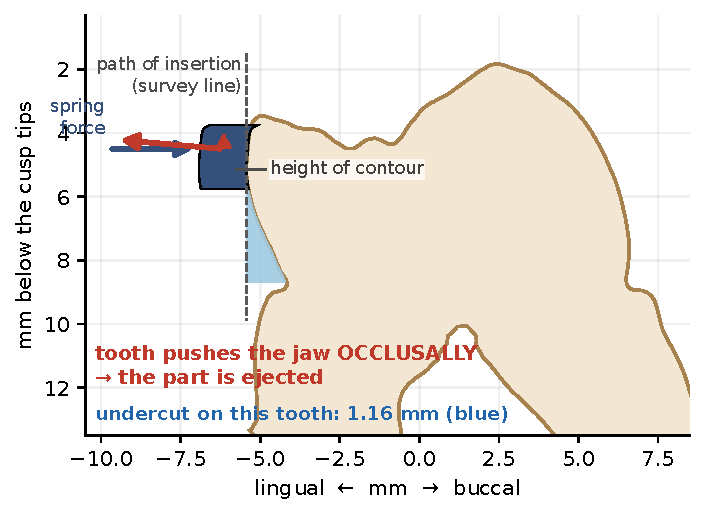
\includegraphics[width=\linewidth]{mech_eject}\caption{Jaw above the lingual height of contour of the first molar.}\end{subfigure}\hfill
\begin{subfigure}[t]{0.325\textwidth}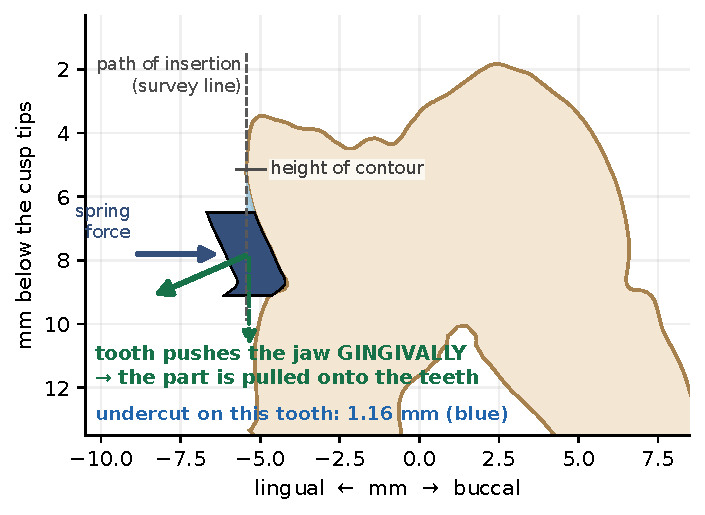
\includegraphics[width=\linewidth]{mech_seat}\caption{Same molar, jaw below it: the same spring seats the part.}\end{subfigure}\hfill
\begin{subfigure}[t]{0.325\textwidth}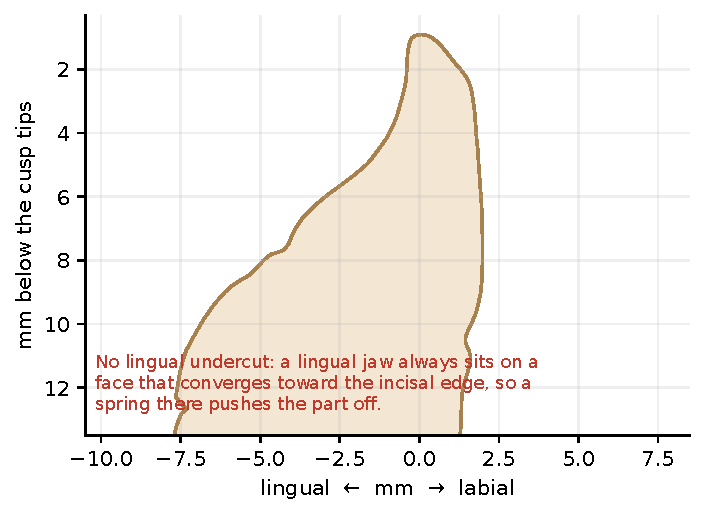
\includegraphics[width=\linewidth]{mech_incisor}\caption{Lower central incisor: the lingual face only widens toward the gum.}\end{subfigure}
\caption{Real sections through \texttt{Teeth\_02}, perpendicular to the arch. Solid arrow: force
of the tooth on the jaw; dashed: its component along the path of insertion.}
\label{fig:mech}
\end{figure}

\Cref{fig:undercut} and \cref{tab:survey} list the undercut on every tooth. Three things follow:
\begin{itemize}
\item \textbf{Molars retain lingually.} First and second molars have
\SIrange{0.3}{1.2}{\milli\metre} of lingual undercut and only \SIrange{0.03}{0.13}{\milli\metre}
buccally. The buccal jaw of any clamp is therefore a rigid \emph{reciprocal} arm that only takes
the reaction force; it cannot hold the part by itself.
\item \textbf{Incisors and canines have no lingual undercut at all.} This is the root cause of the
slipping incisor attachment, independent of how hard the screws are tightened.
\item \textbf{The numbers depend on the path of insertion.} The left/right difference is partly
the tilt of the model. Tilting the path moves undercut from one face to the other; choose it on
the subject's scan so that both molars get \SIrange{0.3}{0.5}{\milli\metre} lingually, then block
out anything deeper.
\end{itemize}

\begin{figure}[H]
\centering
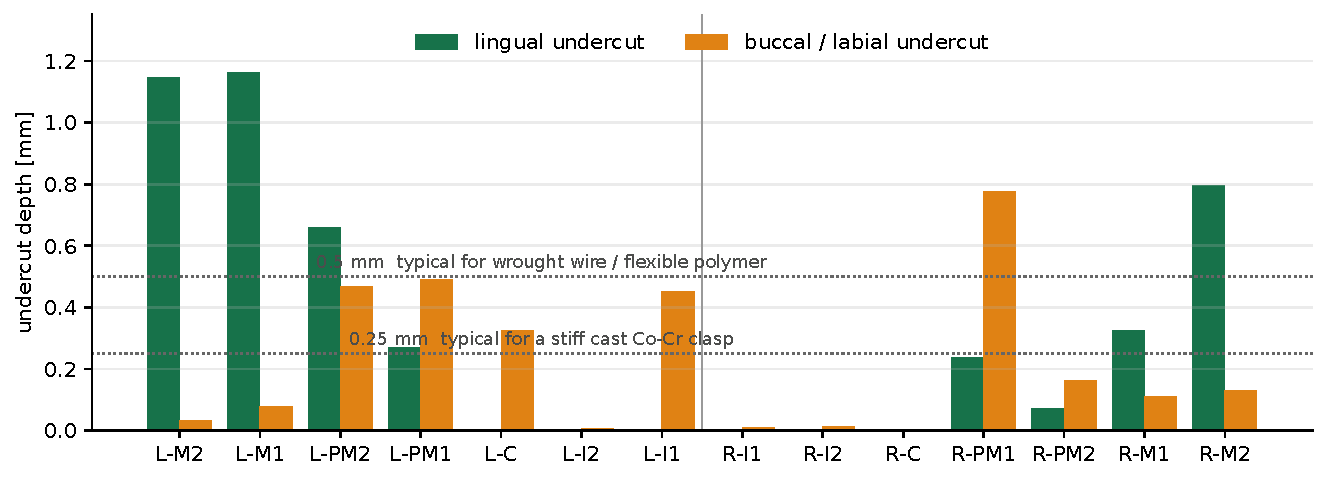
\includegraphics[width=\textwidth]{mech_undercut_bars}
\caption{Usable undercut per tooth for a vertical path of insertion. Dotted lines: typical
engagement depths used for removable-partial-denture clasps.}
\label{fig:undercut}
\end{figure}

\begin{table}[H]
\centering\small
\caption{Undercut depth in mm (output of \texttt{s03\_survey.py}).}\label{tab:survey}
\begin{tabular}{l S[table-format=1.2] S[table-format=1.2] S[table-format=1.2] S[table-format=1.2]}
\toprule
& \multicolumn{2}{c}{left} & \multicolumn{2}{c}{right}\\
\cmidrule(lr){2-3}\cmidrule(lr){4-5}
tooth & {lingual} & {buccal} & {lingual} & {buccal}\\
\midrule
\inputrows{generated/survey_table.tex}
\bottomrule
\end{tabular}
\end{table}

\paragraph{Limits of the model.} The intraoral scan closes the gaps between teeth below the
contact points, so the interproximal undercuts that Adams clasps and resin relines use in a real
mouth do not appear in these numbers. The gingiva is part of the model, so the ``gingival margin''
is where the scanned gum starts.

% This file is part of JTS-MM (https://github.com/paulotto/jts-mm).
% SPDX-FileCopyrightText: 2026 Paul-Otto Müller
% SPDX-License-Identifier: CC-BY-4.0

\section{Design rules common to all concepts}\label{sec:principles}
\begin{enumerate}[label=\textbf{R\arabic*}]
\item \textbf{Put the spring on the lingual side of the molars}, pressing below the lingual height
of contour. The buccal jaw is rigid and only reciprocates.
\item \textbf{Keep the reference rigid and the spring separate.} The marker is only as still as
the part it is mounted on. Whatever defines the position (rests, reciprocal jaw, frame) should
not flex; the spring only supplies preload. A preloaded rigid contact does not move until the
disturbing force exceeds the preload.
\item \textbf{Use rests as the vertical datum.} Small pads on the marginal ridges next to the
embrasure between the second premolar and first molar define how far the part sits down, the way
occlusal rests do on a partial denture. They replace the incisal stop of the old design.
\item \textbf{Cross the bite only at embrasures}, and check those points with articulating paper.
Everything else stays off the occlusal surfaces, so chewing kinematics are not changed.
\item \textbf{Block out, then relieve.} On the model, fill undercuts deeper than the target
engagement (\SIrange{0.3}{0.5}{\milli\metre} for polymers, \SI{0.4}{\milli\metre} for the
\SI{0.9}{\milli\metre} arch wire) and add \SIrange{0.1}{0.2}{\milli\metre} relief on every
surface that should not touch.
\item \textbf{Reline with resin, and give it something to hold.} A thin layer of light- or
cold-curing resin captures the real tooth shape, including the interproximal undercuts. Resin does
not bond to PETG, PA12 or TPU: design holes, grooves or undercut slots into the printed part.
\item \textbf{Materials for participants.} FDM PETG, PA12 and TPU are fine for bench prototypes
on a printed model but are not certified for intraoral use. Parts worn by participants should be
printed in a certified splint resin (e.g.\ a Class~IIa occlusal-splint resin; flexible grades
exist as an alternative to TPU) and fitted under dental supervision, as covered by the ethics
approval. Both stainless wire grades in \cref{sec:procurement} contain about \SI{8}{\percent}
nickel: ask about nickel allergy.
\end{enumerate}

% This file is part of JTS-MM (https://github.com/paulotto/jts-mm).
% SPDX-FileCopyrightText: 2026 Paul-Otto Müller
% SPDX-License-Identifier: CC-BY-4.0

\section{Overview of the five concepts}\label{sec:overview}
\begin{figure}[H]
\centering
\newcommand{\ov}[2]{\begin{subfigure}[t]{0.19\textwidth}\centering\includegraphics[width=\linewidth]{render_#1_obl}\caption*{\small #2}\end{subfigure}}
\ov{c1}{1 Snap shell}\hfill\ov{c2}{2 Clothespin jaw}\hfill\ov{c3}{3 Wire clasps}\hfill\ov{c4}{4 Spring arch}\hfill\ov{c5}{5 Rigid + TPU}
\caption{All five concepts on \texttt{Teeth\_02}. Colours: \swatch{cprinted}~printed, conforming;
\swatch{crigid}~rigid frame (reference); \swatch{cspring}~printed spring;
\swatch{ctpu}~TPU; \swatch{cwire}~stainless wire. The black plate stands for the marker.}
\label{fig:overview}
\end{figure}

\begin{table}[H]
\centering\small
\caption{Comparison. Green = favourable, red = the main weakness.}\label{tab:compare}
\begin{tabularx}{\textwidth}{l*{5}{>{\centering\arraybackslash}X}}
\toprule
& 1 Snap shell & 2 Clothespin & 3 Wire clasps & 4 Spring arch & 5 Rigid + TPU\\
\midrule
spring & shell wall & printed C-loop & \SI{0.7}{mm} steel & \SI{0.9}{mm} steel arch & TPU liner\\
parts & \good{1 print} & \good{1 print} & print + wire & print + wire & 2 materials\\
grips & \good{lingual} & \good{lingual} & buccal embrasures & \good{lingual} & \good{lingual}\\
reference rigid? & \bad{no} & \good{yes} & \good{yes} & mostly & \good{yes}\\
preload in session & \bad{creeps} & \bad{creeps} & \good{stable} & \good{stable} & relaxes\\
crosses the bite & 4 embrasures & 2 embrasures & \bad{4 wire crossings} & \good{C/PM1 only} & 2 embrasures\\
effort to first test & \good{lowest} & medium & \bad{wire bending} & medium & \good{low}\\
\bottomrule
\end{tabularx}
\end{table}

% This file is part of JTS-MM (https://github.com/paulotto/jts-mm).
% SPDX-FileCopyrightText: 2026 Paul-Otto Müller
% SPDX-License-Identifier: CC-BY-4.0

\section{The concepts in detail}\label{sec:concepts}
Each concept is shown on the right side of the arch: an overall view, the first molar from the
buccal and from the lingual side, and a section through the first molar. The section is an
editable SVG in \texttt{figures/svg/}; the geometry is in \texttt{stl/} in the coordinate frame of
\texttt{Teeth\_02}, so it drops onto the teeth when imported into the FreeCAD document. The STLs
are concept geometry on a \SI{0.2}{mm} voxel grid, meant as a starting point for CAD, not as
print files.

\newcommand{\conceptfig}[2]{%
\begin{figure}[H]\centering
\begin{subfigure}[b]{0.54\textwidth}\includegraphics[width=\linewidth]{render_#1_obl}\caption{overview}\end{subfigure}\hfill
\begin{subfigure}[b]{0.44\textwidth}\includegraphics[width=\linewidth]{section_#1}\caption{section through the first molar}\end{subfigure}\\[2mm]
\begin{subfigure}[b]{0.49\textwidth}\includegraphics[width=\linewidth,height=45mm,keepaspectratio]{render_#1_molB}\caption{first molar, buccal side}\end{subfigure}\hfill
\begin{subfigure}[b]{0.49\textwidth}\includegraphics[width=\linewidth,height=45mm,keepaspectratio]{render_#1_molL}\caption{first molar, lingual side}\end{subfigure}
\caption{#2}\label{fig:#1}\end{figure}}

% ---------------------------------------------------------------------------
\subsection{Concept 1: snap shell}
\conceptfig{c1}{Concept 1. One conforming shell: lingual flange on all teeth, buccal reciprocal arms on both molars, bridges over the embrasures, labial bar with the marker stem.}
\textbf{Principle.} Like a partial clear aligner: the lingual flange snaps under the lingual height
of contour of the molars; the wall itself is the spring.

\textbf{Parameters.} Wall \SI{1.5}{mm} (PETG/PA12) or \SIrange{1.0}{1.2}{mm} (splint resin);
flange from \SI{1.4}{mm} below the lingual cusp tips to \SIrange{1}{1.5}{mm} onto the lingual
gingiva; buccal arms \SI{1.3}{mm}, above the buccal height of contour; embrasure bridges
\SI{\ge1.5}{mm} wide, \SI{1.0}{mm} thick; labial bar \SI{1.6}{mm} on the cervical half of the
incisors and canines.

\textbf{Build.}
\begin{enumerate}
\item Survey and block out the molar lingual undercut to \SI{0.3}{mm} (PETG) or
\SI{0.5}{mm} (flexible splint resin); relieve all other surfaces by \SI{0.1}{mm}.
\item Offset the blocked-out model by the wall thickness (e.g.\ Meshmixer ``offset'', Blender
``solidify'', or start from \texttt{stl/c1\_printed.stl}) and trim to the outline in \cref{fig:c1}.
\item Print in splint resin (SLA/DLP). In FDM, orient the part so that the flange bends
\emph{within} the layer plane, not across layers.
\item Fit on the printed model, then reline the lingual flange with resin through retention holes.
\end{enumerate}
\textbf{Watch out.} Spring and reference are the same part: whenever the flange flexes, the marker
moves. Preload depends directly on print accuracy.

% ---------------------------------------------------------------------------
\subsection{Concept 2: clothespin jaw}
\conceptfig{c2}{Concept 2. Rigid frame (lingual bar, buccal jaw, bridge over the PM2/M1 embrasure, labial bar) and a compliant lingual jaw hung on a C-loop flexure, an intraoral version of a printed spring clamp.}
\textbf{Principle.} The lingual jaw is carried by a C-shaped loop spring that sits next to the
tongue, below the occlusal plane. It is printed over-closed; inserting the clamp opens it over the
height of contour, and it springs back into the undercut.

\textbf{Parameters.} Loop radius $R=\SI{3.0}{mm}$ to the wall centre, wall $t=\SI{0.8}{mm}$ (two
\SI{0.4}{mm} extrusion lines), width $w=\SI{5.5}{mm}$ along the arch, \SI{270}{\degree} arc,
loop centre at the contact height ($e=0$), over-closure \SI{0.2}{mm}; lingual jaw \SI{1.2}{mm} from
$h=6.3$ to $9.3$; rigid buccal jaw \SI{1.4}{mm}. This gives \SI{\approx1.5}{N} preload and
\SI{\approx3.7}{N} while passing a \SI{0.3}{mm} undercut, at \SI{\approx1.0}{\percent} peak strain
(\cref{sec:loop}). Dimensioned drawings: \cref{fig:drw_c2}.

\textbf{Build.}
\begin{enumerate}
\item Design the loop module (jaw + loop + foot) as a separate clip-in part with a dovetail on the
lingual bar. It can then be printed flat with the loop in the layer plane, and swapped to change
the force.
\item Print the frame rigid (PETG, \SI{100}{\percent} infill, or splint resin).
\item Measure the jaw force with a spring scale at \SI{0.2}{mm} opening and at \SI{0.5}{mm}. Adjust
the width $w$ (force $\propto w$), not the wall thickness: $t$ sets the strain, $w$ sets the force.
\item Add a small tab on the lingual jaw so it can be pulled open with a probe for removal.
\end{enumerate}
\textbf{Watch out.} Printed polymer flexures relax at \SI{37}{\celsius} under constant strain:
measure the force again after \SI{30}{min} in warm water. A loop of $R=\SI{3}{mm}$ reaches about
\SI{7}{mm} lingual of the tooth, into the tongue space; the two-loop variant in \cref{tab:loop}
is more compact.

% ---------------------------------------------------------------------------
\subsection{Concept 3: wire clasps}
\conceptfig{c3}{Concept 3. Rigid printed lingual plate with occlusal rests and an Adams clasp of \SI{0.7}{mm} spring-hard stainless steel around each first molar.}
\textbf{Principle.} The classic removable-retainer solution. The two arrowheads of each Adams
clasp engage the mesio- and disto-buccal undercuts below the contact points, which exist even where
the buccal face itself has only \SI{0.1}{mm}. The spring is metal, so the preload does not creep.

\textbf{Parameters.} \SI{0.7}{mm} hard stainless on molars (\SI{0.6}{mm} on premolars); arrowheads
\SIrange{0.5}{1}{mm} into the undercut; bridge about \SI{1}{mm} off the buccal surface at mid-crown
height; tags cross the embrasures resting on the marginal ridges and end in the plate with
retention bends.

\textbf{Build.}
\begin{enumerate}
\item On a printed or stone model, trim a small notch (about \SI{0.5}{mm}) at the two arrowhead
sites just below the contact points; this is where the arrowheads will sit.
\item Bend the clasp (a dental technician does this in minutes; any orthodontic lab textbook
shows the sequence). Alternative without bending: prefabricated ball clasps in the buccal
embrasures.
\item Print the lingual plate with channels for the tags; fix the tags with cold-cure resin.
\item Adjust retention with pliers at the arrowheads, never by heating the wire.
\end{enumerate}
\textbf{Watch out.} The wire crosses the occlusal embrasures in four places: check the bite.

% ---------------------------------------------------------------------------
\subsection{Concept 4: spring arch (inside push)}
\conceptfig{c4}{Concept 4. A \SI{0.9}{mm} stainless arch behind the teeth (grey: mounted, orange: free shape, pre-spread \SI{0.7}{mm} per side) pushes resin-relined pads outward under the lingual heights of contour of both molars. Rigid anterior yoke and labial bar carry the marker.}
\textbf{Principle.} The expander principle, turned into a clamp: one U-shaped arch, bent slightly
too wide, pushes both molar pads outward into the deepest undercuts in the mouth. The pads seat
themselves (\cref{fig:mech}b). The front of the arch is bridged by the rigid yoke; only the two
legs (\SI{\approx18}{mm} from canine to first molar) act as springs.

\textbf{Parameters.} \SI{0.9}{mm} spring-hard stainless; pre-spread \SI{0.7}{mm} per side; lingual
undercut blocked out to \SI{0.4}{mm}; result \SI{\approx2.3}{N} preload per side, peak stress
\SI{\approx0.9}{GPa} (\cref{sec:springs}). Optional omega loop in each leg for more margin and
adjustability.

\textbf{Build.}
\begin{enumerate}
\item Block out the molar lingual undercut to \SI{0.4}{mm} on the model.
\item Bend the arch on the model, \SI{1}{mm} off the lingual gingiva, from the first-molar pad on
one side to the other; finish the leg ends as small retention loops.
\item Print the pads (splint resin or PETG) with a channel for the loop; fix with cold-cure resin;
reline the tooth side.
\item Activate: open each leg so the distance between the pad contact points is
\SI{1.4}{mm} larger than on the model. Check with a spring scale: \SI{\approx2}{N} per side at
\SI{0.7}{mm}.
\item Remove by pinching the two legs toward each other.
\end{enumerate}
\textbf{Watch out.} Do not pre-spread more than about \SI{1}{mm} or leave deeper undercuts: the
wire then yields (\cref{fig:springs}). Pull-off force is only \SI{\approx1}{N} per side; if that is
not enough, combine with concept~3.

% ---------------------------------------------------------------------------
\subsection{Concept 5: rigid clamp with TPU liner}
\conceptfig{c5}{Concept 5. Hard buccal jaw and hard rest over the PM2/M1 embrasure define the position; a \SIrange{1.5}{2}{mm} TPU liner on the rigid lingual jaw provides the preload.}
\textbf{Principle.} Nothing rigid flexes. The TPU liner is compressed while the clamp passes the
height of contour and expands back into the undercut. TPU is roughly 30--100$\times$ softer than
PETG, so it must be loaded in compression, not used as a clasp arm.

\textbf{Parameters.} Liner \SIrange{1.5}{2}{mm}, TPU 85A--95A, \textbf{ribbed} (e.g.\ four vertical
ribs, about \SI{35}{\percent} solid); interference \SIrange{0.1}{0.2}{mm}; lingual undercut
blocked out to \SI{0.3}{mm}. \Cref{tab:tpu} shows why solid liners are a bad idea: a solid pad
gives tens of newtons for a tenth of a millimetre.

\textbf{Build.}
\begin{enumerate}
\item Print the rigid frame (PETG or splint resin) with a dovetail slot in the lingual jaw.
\item Print the TPU liner as a clip-in insert with the ribs running occluso-gingivally, so the
tooth slides along them on insertion. Dual-material printing with an interlocking pattern also
works.
\item Reline the hard buccal jaw and the rest with resin; do not reline the TPU.
\item Set the interference by the insert thickness; measure pull-off with a spring scale.
\end{enumerate}
\textbf{Watch out.} TPU relaxes under constant compression; re-check the force after a typical
session length. A flexible splint resin is the certified alternative for participants.

% This file is part of JTS-MM (https://github.com/paulotto/jts-mm).
% SPDX-FileCopyrightText: 2026 Paul-Otto Müller
% SPDX-License-Identifier: CC-BY-4.0

\section{The parts on their own}\label{sec:parts}
The same geometry as in \cref{sec:concepts}, without the teeth: an overall view, the view from
above (occlusal), and the right first-molar region from the lingual and from the buccal side.

\newcommand{\partsfig}[2]{%
\begin{figure}[H]\centering
\begin{subfigure}[b]{0.5\textwidth}\includegraphics[width=\linewidth]{render_#1_solo_obl}\caption{overview}\end{subfigure}\hfill
\begin{subfigure}[b]{0.34\textwidth}\includegraphics[width=\linewidth]{render_#1_solo_top}\caption{from above}\end{subfigure}\\[1mm]
\begin{subfigure}[b]{0.49\textwidth}\includegraphics[width=\linewidth,height=42mm,keepaspectratio]{render_#1_solo_detL}\caption{right M1 region, lingual}\end{subfigure}\hfill
\begin{subfigure}[b]{0.49\textwidth}\includegraphics[width=\linewidth,height=42mm,keepaspectratio]{render_#1_solo_detB}\caption{right M1 region, buccal}\end{subfigure}
\caption{#2}\label{fig:parts_#1}\end{figure}}

\partsfig{c1}{Concept 1, snap shell (one part).}
\partsfig{c2}{Concept 2, clothespin jaw: rigid frame \swatch{crigid} and loop module \swatch{cspring}.}
\partsfig{c3}{Concept 3, rigid lingual plate with rests and two Adams clasps.}
\partsfig{c4}{Concept 4, rigid yoke and labial bar, stainless arch and relined pads.}
\partsfig{c5}{Concept 5, rigid frame and TPU liners \swatch{ctpu}.}

% This file is part of JTS-MM (https://github.com/paulotto/jts-mm).
% SPDX-FileCopyrightText: 2026 Paul-Otto Müller
% SPDX-License-Identifier: CC-BY-4.0

\section{Dimensioned drawings and FreeCAD recipe}\label{sec:drawings}
\subsection{How to build the parts in FreeCAD}\label{sec:freecad}
Every part is either a \emph{profile swept along a curve that follows the teeth} (bars, jaws, pads,
wires) or a \emph{conforming shell} (the flange of concept~1 and the plate of concept~3). The folder
\texttt{cad/} contains everything needed to place the profiles:
\begin{itemize}
\item \texttt{import\_reference\_geometry.FCMacro}: run it with the FCStd open. It creates
\begin{description}[style=nextline,leftmargin=2em]
\item[\texttt{REF\_curves}] B-spline sweep paths on the tooth surface (offset by \SI{0.05}{mm},
interdental notches closed with a \SI{2.5}{mm} rolling ball), the wire centrelines of concepts 3
and 4, and the arch centreline.
\item[\texttt{REF\_sections}] one sketch per station, placed in the section plane with
\textbf{sketch $x = n$} (positive buccal) and \textbf{sketch $y = h$} (from the lowest cusp tip,
positive toward the gum). The tooth outline is included as construction geometry. The
coordinates in the section drawings below can be typed in directly. (In FreeCAD the model's gum
side is $+z$, so the sketch appears upside down relative to the drawings.)
\item[\texttt{REF\_path\_starts}] one sketch at the start of every sweep path, same orientation,
origin on the path: draw the profile relative to the path there.
\end{description}
\item The same curves as DXF (one file each and \texttt{all\_reference\_geometry.dxf}) and CSV
($x,y,z,s$), and \texttt{stations.csv} with position, tangent and normal of every station.
\end{itemize}

\paragraph{Recipe.}
\begin{enumerate}
\item Open the FreeCAD file with the teeth model
(\texttt{parts/teeth\_attachment/teeth\_attachment.FCStd}), run the macro. Optionally import the concept
STL from \texttt{stl/} as a visual check; it sits on the teeth.
\item \textbf{Long parts} (lingual bar, labial bar, yoke): open the matching \texttt{START\_} sketch,
draw the profile from the section drawing \emph{relative to the path} (e.g.\ lingual bar: rectangle
$x\in[-2.0,\,0]$, $y\in[-1.4,\,+1.4]$), then \emph{Part $\rightarrow$ Sweep}: profile = sketch,
path = the \texttt{REF\_} curve, \emph{Solid} on, \emph{Frenet} off. This was tested on the
lingual bar path.
\item \textbf{Short parts on one tooth} (jaws, pads, loop module, TPU insert, rests): draw the
profile in \texttt{SEC\_M1\_mid\_R} and \emph{Pad} it symmetrically by its length along the arch
(from the plan view and parameter table). Over \SIrange{7}{9}{mm} the molar face is straight to
about \SI{0.1}{mm}; the resin reline takes up the rest.
\item \textbf{Wires}: sweep a circle of the wire diameter along \texttt{REF\_c4\_wire\_mounted} or
\texttt{REF\_c3\_adams\_*} (for visualisation and clearance checks only; the real wire is bent on
the model).
\item \textbf{Conforming shells} (concepts 1 and 3): start from \texttt{stl/c1\_printed.stl} /
\texttt{stl/c3\_rigid.stl}, or offset a blocked-out tooth model (Meshmixer, Blender) by the wall
thickness; a parametric sweep cannot follow the crown shape.
\item Mirror left/right with \emph{Part $\rightarrow$ Mirror} about the plane through
\texttt{REF\_ref\_centreline\_h6p0} at $s=0$ only if the subject's arch is symmetric enough; the
reference curves exist for both sides.
\item Fuse, add retention holes for the resin (Ø\SI{1.2}{mm}, \SI{3}{mm} pitch) and the
\SI{0.1}{mm} relief on non-contacting faces, export STL.
\end{enumerate}

\subsection{Reference dimensions of the dental arch}
\begin{figure}[H]\centering
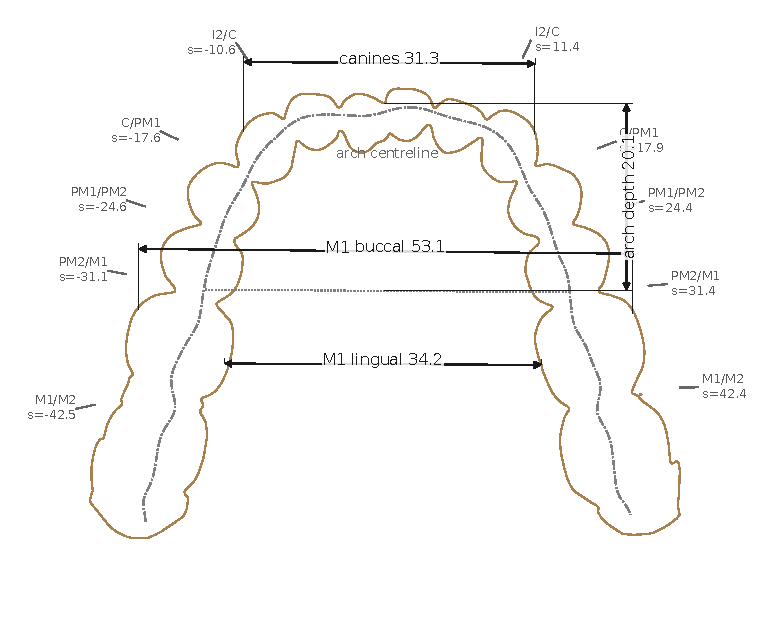
\includegraphics[width=0.72\textwidth]{drw_ref_plan}
\caption{Occlusal plan of \texttt{Teeth\_02} (section at $h=6.5$), $X=x-x_\text{midline}$, anterior
at the top. Stations $s$ are arc lengths along the centreline; all drawings refer to them.}
\label{fig:drw_ref}
\end{figure}
\begin{table}[H]\centering\small
\caption{Measured on \texttt{Teeth\_02} (\texttt{s09\_drawings.py}).}\label{tab:refdims}
\begin{tabular}{l S[table-format=2.1]}
\toprule dimension & {mm}\\ \midrule
\inputrows{generated/ref_dims.tex}
\bottomrule
\end{tabular}
\end{table}

\newcommand{\paramtable}[2]{%
\begin{table}[H]\centering\small\caption{#2}\label{tab:params_#1}
\begin{tabularx}{\textwidth}{X l l}\toprule parameter & key in \texttt{params.py} & value [mm, deg]\\ \midrule
\inputrows{generated/params_#1.tex}
\bottomrule\end{tabularx}\end{table}}

\subsection{Common parts}
\begin{figure}[H]\centering
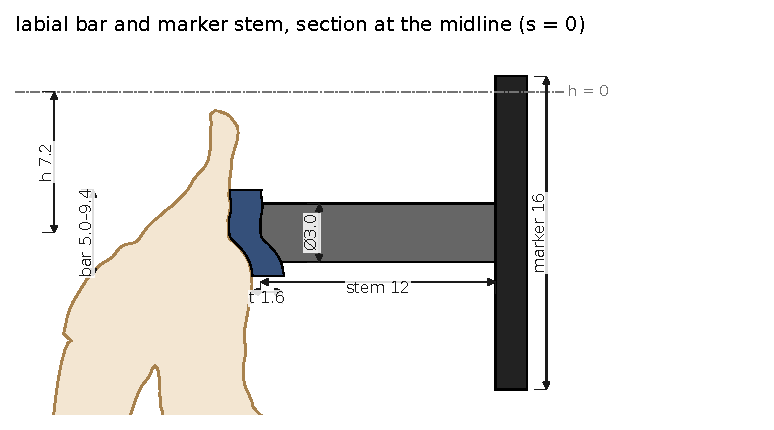
\includegraphics[width=0.8\textwidth]{drw_common_marker}
\caption{Labial bar and marker stem at the midline. The labial bar is the same in all concepts;
sweep its profile along \texttt{REF\_path\_labial\_h7p2} over $s=\pm16.5$.}
\label{fig:drw_common}
\end{figure}
\paramtable{common}{Common parameters.}

\subsection{Concept 1: snap shell}
\begin{figure}[H]\centering
\begin{subfigure}[b]{0.48\textwidth}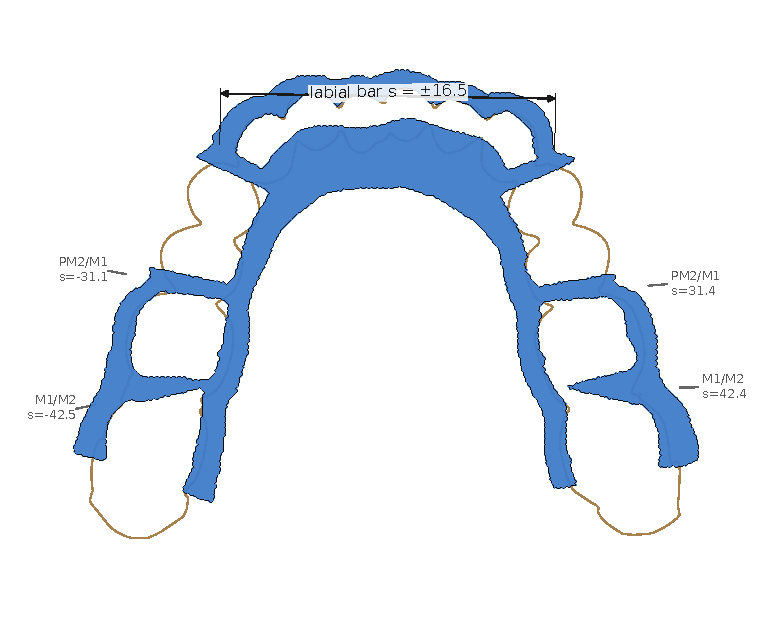
\includegraphics[width=\linewidth]{drw_c1_plan}\caption{plan}\end{subfigure}\hfill
\begin{subfigure}[b]{0.48\textwidth}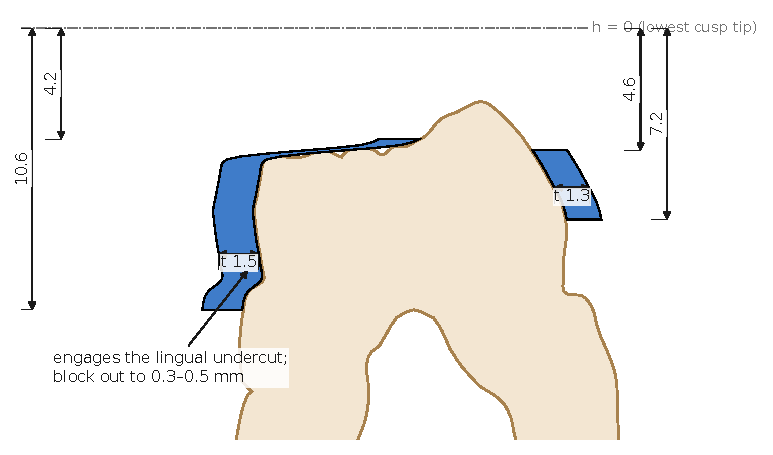
\includegraphics[width=\linewidth]{drw_c1_section}\caption{section at the right M1}\end{subfigure}
\caption{Concept 1. Build the shell from the STL or by offsetting (see recipe); the section gives the thicknesses and extents.}\label{fig:drw_c1}
\end{figure}
\paramtable{c1}{Concept 1 parameters.}

\subsection{Concept 2: clothespin jaw}
\begin{figure}[H]\centering
\begin{subfigure}[b]{0.46\textwidth}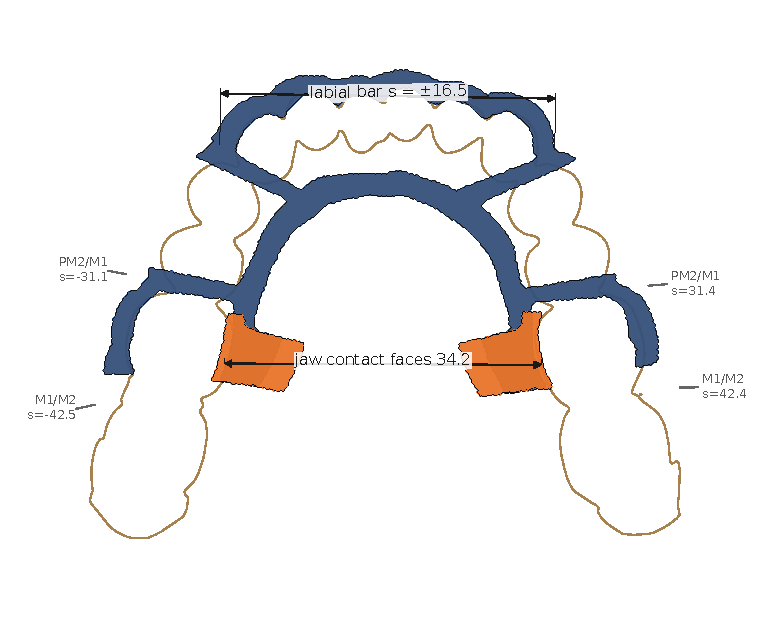
\includegraphics[width=\linewidth]{drw_c2_plan}\caption{plan}\end{subfigure}\hfill
\begin{subfigure}[b]{0.52\textwidth}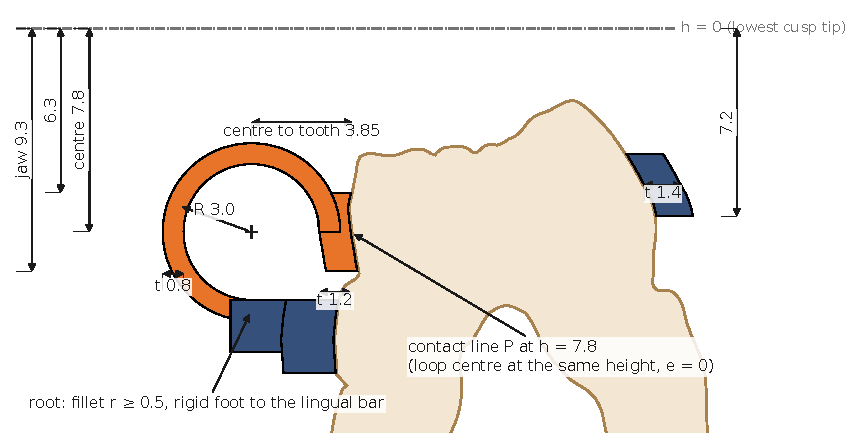
\includegraphics[width=\linewidth]{drw_c2_section}\caption{section at the right M1}\end{subfigure}\\[2mm]
\begin{subfigure}[b]{\textwidth}\centering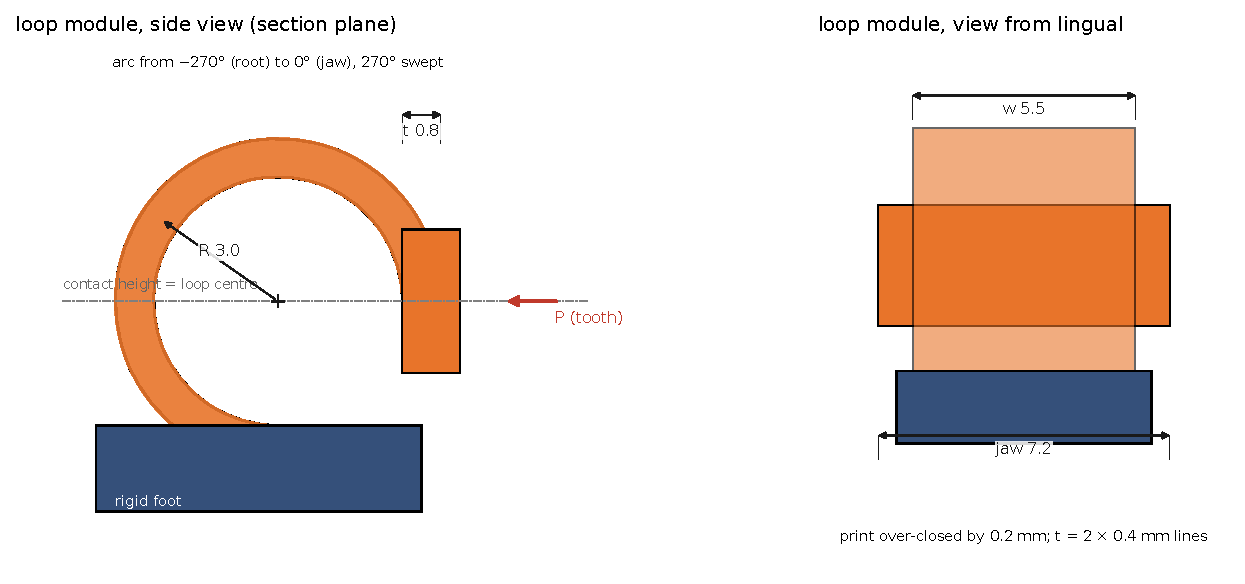
\includegraphics[width=0.9\linewidth]{drw_c2_loop}\caption{loop module (clip-in part)}\end{subfigure}
\caption{Concept 2. Lingual bar: sweep a \SI{2.0}{mm}$\times$\SI{2.8}{mm} rectangle along
\texttt{REF\_path\_lingual\_bar\_h11p8}. Buccal jaw, loop module and foot: pad from
\texttt{SEC\_M1\_mid\_R}. Loop sizing: \cref{sec:loop}.}\label{fig:drw_c2}
\end{figure}
\paramtable{c2}{Concept 2 parameters.}

\subsection{Concept 3: wire clasps}
\begin{figure}[H]\centering
\begin{subfigure}[b]{0.46\textwidth}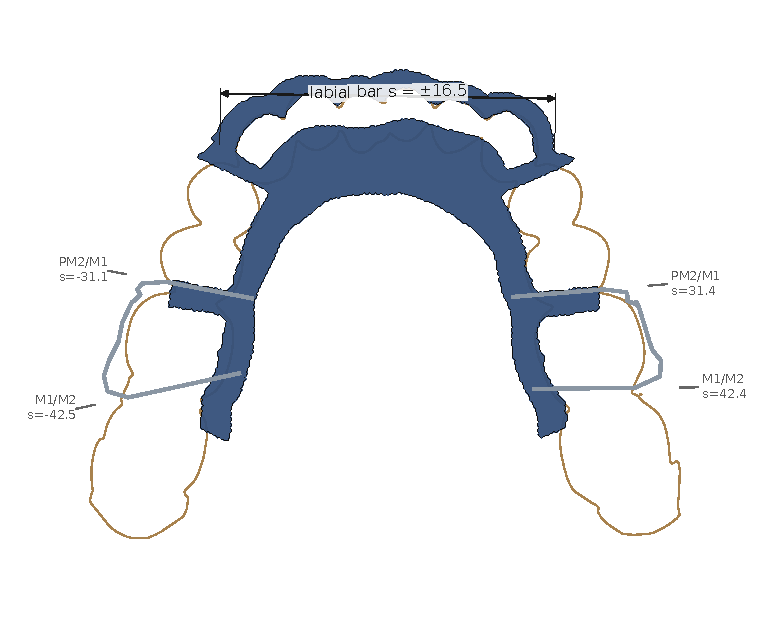
\includegraphics[width=\linewidth]{drw_c3_plan}\caption{plan}\end{subfigure}\hfill
\begin{subfigure}[b]{0.50\textwidth}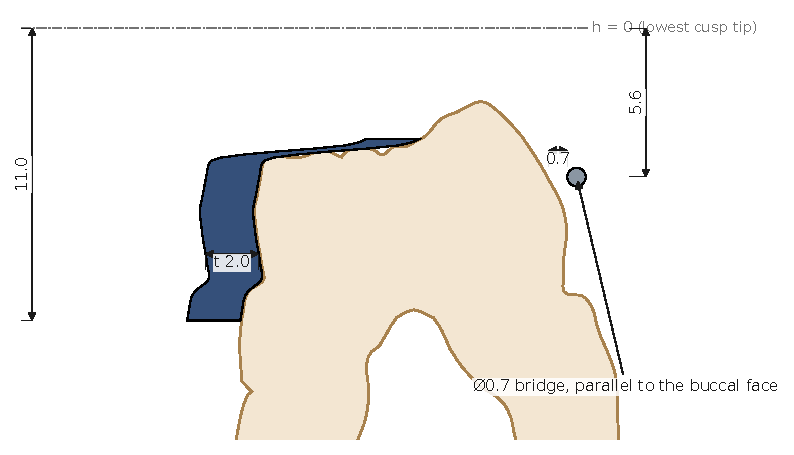
\includegraphics[width=\linewidth]{drw_c3_section}\caption{section at the right M1}\end{subfigure}\\[2mm]
\begin{subfigure}[b]{\textwidth}\centering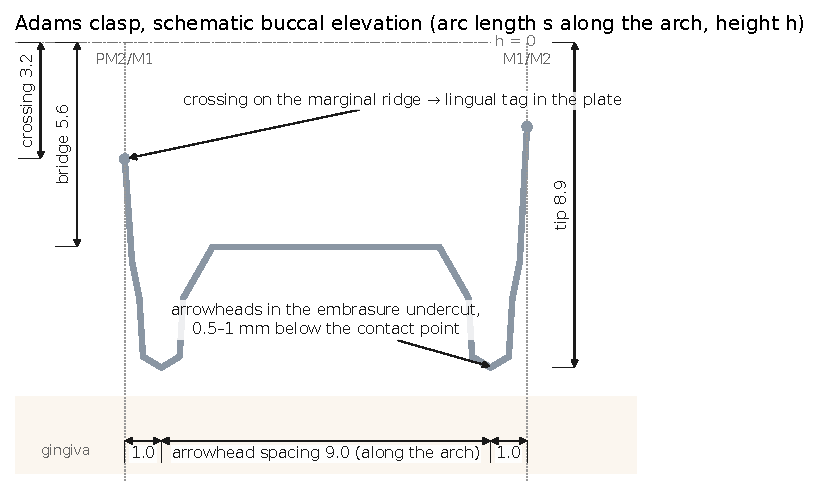
\includegraphics[width=0.8\linewidth]{drw_c3_adams}\caption{Adams clasp}\end{subfigure}
\caption{Concept 3. The plate is a conforming shell; the clasp is bent on the model following (c) and
\texttt{REF\_c3\_adams\_*}.}\label{fig:drw_c3}
\end{figure}
\paramtable{c3}{Concept 3 parameters.}

\subsection{Concept 4: spring arch}
\begin{figure}[H]\centering
\begin{subfigure}[b]{0.48\textwidth}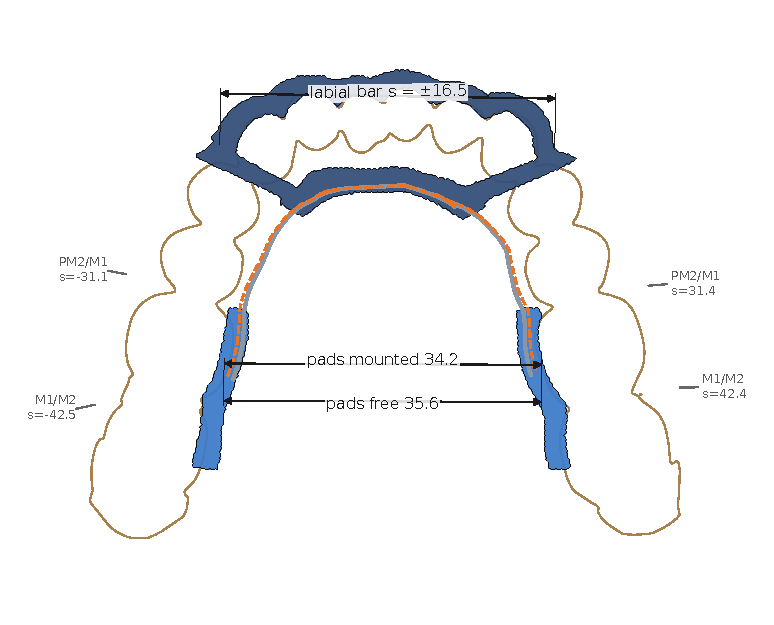
\includegraphics[width=\linewidth]{drw_c4_plan}\caption{plan: wire mounted (grey) and free (dashed)}\end{subfigure}\hfill
\begin{subfigure}[b]{0.48\textwidth}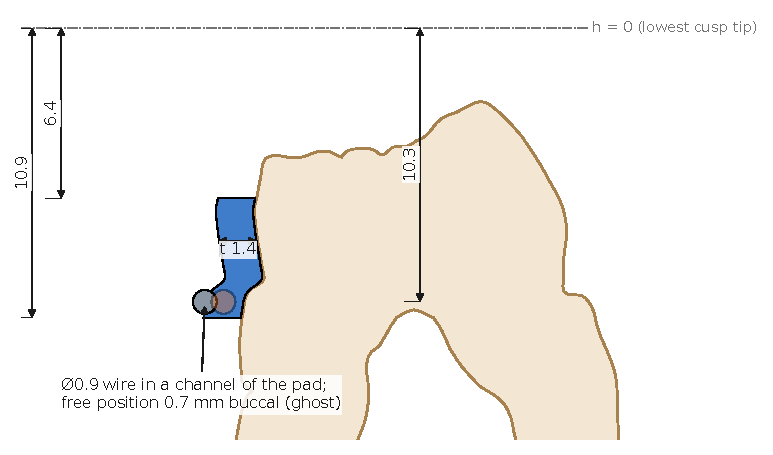
\includegraphics[width=\linewidth]{drw_c4_section}\caption{section at the right M1}\end{subfigure}
\caption{Concept 4. Bend the wire to \texttt{REF\_c4\_wire\_free} (the mounted shape spread by
\SI{0.7}{mm} per side); pads: pad the section profile over the M1 and M2 station ranges.}\label{fig:drw_c4}
\end{figure}
\paramtable{c4}{Concept 4 parameters.}

\subsection{Concept 5: rigid clamp with TPU liner}
\begin{figure}[H]\centering
\begin{subfigure}[b]{0.46\textwidth}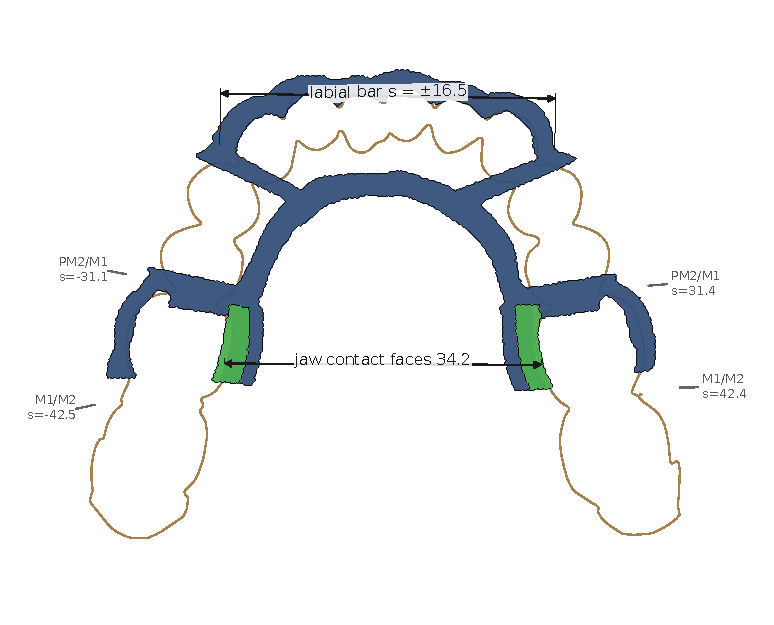
\includegraphics[width=\linewidth]{drw_c5_plan}\caption{plan}\end{subfigure}\hfill
\begin{subfigure}[b]{0.50\textwidth}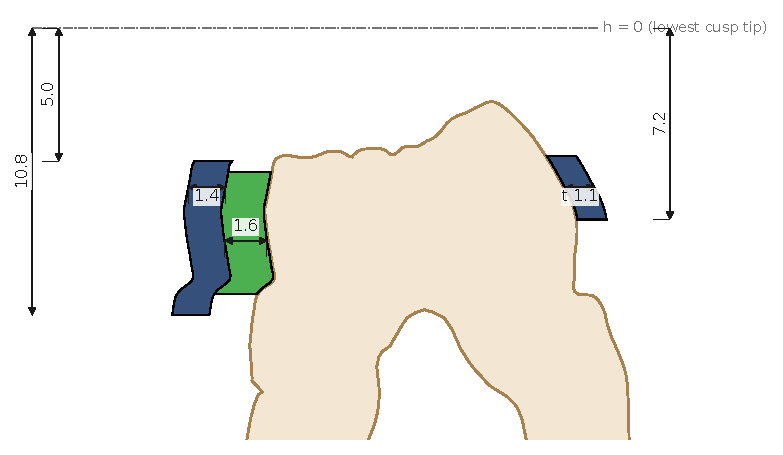
\includegraphics[width=\linewidth]{drw_c5_section}\caption{section at the right M1}\end{subfigure}\\[2mm]
\begin{subfigure}[b]{\textwidth}\centering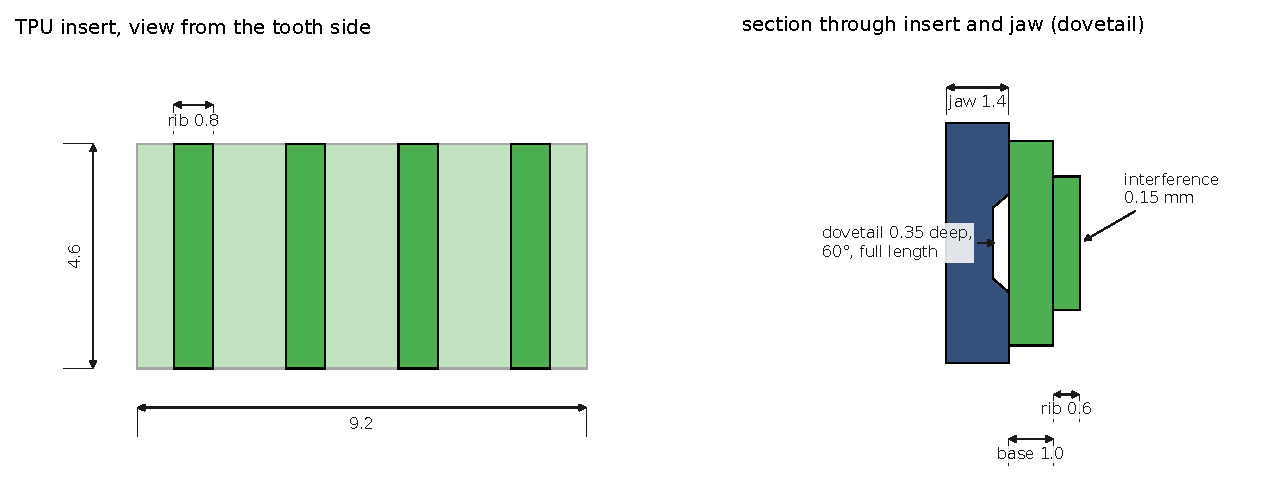
\includegraphics[width=0.85\linewidth]{drw_c5_insert}\caption{TPU insert and dovetail}\end{subfigure}
\caption{Concept 5. The TPU insert slides into a dovetail in the rigid jaw; interference is set by
the insert thickness.}\label{fig:drw_c5}
\end{figure}
\paramtable{c5}{Concept 5 parameters.}

% This file is part of JTS-MM (https://github.com/paulotto/jts-mm).
% SPDX-FileCopyrightText: 2026 Paul-Otto Müller
% SPDX-License-Identifier: CC-BY-4.0

\section{Spring design mathematics}\label{sec:springs}
All springs in this document are sized with the same few relations. The scripts evaluate them
(\texttt{s08\_springs.py}, inputs at the top and in \texttt{params.py}); the formulas are given here
so they can be checked and applied by hand. Verify every spring with a spring scale before use.

\subsection{Method: strain first, force second}\label{sec:method}
Every clamp in this document works the same way. The spring is printed or bent so that, mounted, it
is deflected by a \emph{preload} $\delta_0$ (over-closure or pre-spread). While the part is pushed
over the height of contour it is deflected further, to
\begin{equation}
\delta_\text{max} = \delta_0 + u ,
\end{equation}
where $u$ is the undercut that the jaw must pass (after block-out). Two requirements follow:
\begin{enumerate}
\item \textbf{Strain.} At $\delta_\text{max}$ the peak strain must stay below what the material
tolerates repeatedly: about \SI{1}{\percent} for PETG and rigid splint resins, \SI{1.5}{\percent}
for PA12, \SI{0.5}{\percent} for spring-hard stainless steel. For every bending spring the peak
strain depends only on geometry and deflection, \emph{not} on the width or on $E$. So the strain
limit fixes the \emph{shape} (length, radius, wall thickness).
\item \textbf{Force.} The preload $F_0=k\,\delta_0$ sets the retention. The stiffness $k$ is
proportional to the width of the spring, so once the shape is fixed, the width sets the force.
\end{enumerate}

\paragraph{Energy bound.} A spring of volume $V$ can store at most
$U=\eta\,V\,E\,\varepsilon^2/2$, where $\eta$ is a shape efficiency ($1/9$ for a straight
rectangular cantilever, $1/3$ for constant bending moment, $1$ for uniform compression). Since
$U = F_\text{max}\delta_\text{max}/2$,
\begin{equation}
V_\text{min} = \frac{F_\text{max}\,\delta_\text{max}}{\eta\,E\,\varepsilon_\text{allow}^2}.
\label{eq:energy}
\end{equation}
\Cref{tab:energy} evaluates this for \SI{3}{N} at \SI{0.5}{mm}. It explains in one line why dental
clasps are made of metal: a printed polymer spring needs roughly \SIrange{35}{70}{mm^3} of flexing
material per jaw, a steel wire about \SI{3}{mm^3}.

\begin{table}[H]\centering\small
\caption{Minimum spring volume for $F_\text{max}=\SI{3}{N}$ at $\delta_\text{max}=\SI{0.5}{mm}$, \cref{eq:energy}.}\label{tab:energy}
\begin{tabular}{l l S[table-format=1.2] S[table-format=2.1] S[table-format=2.0]}
\toprule
material & loading & {$\eta$} & {$\varepsilon_\text{allow}$ [\%]} & {$V_\text{min}$ [mm$^3$]}\\
\midrule
\inputrows{generated/energy_table.tex}
\bottomrule
\end{tabular}
\end{table}

\paragraph{Pull-off force.} A jaw pressing with normal force $N$ on a face inclined by $\alpha$ to
the path of insertion (from the undercut depth $u$ over the engaged height $z$,
$\tan\alpha=u/z$) must be pushed outward to remove the part. With friction coefficient $\mu$, a
force balance along and across the face gives
\begin{equation}
F_\text{pull-off} = N\,\frac{\tan\alpha+\mu}{1-\mu\tan\alpha}, \qquad N = k\,(\delta_0+u)
\label{eq:pulloff}
\end{equation}
per jaw. For small $\alpha$ this is simply $N(\alpha+\mu)$: retention comes from the undercut and
from friction in roughly equal parts.

% ---------------------------------------------------------------------------
\subsection{Printed C-loop (concept 2)}\label{sec:loop}
\paragraph{Model.} The loop is a curved cantilever: a circular arc of radius $R$ (to the wall
centre), wall thickness $t$ and width $w$, clamped at the root angle $a_1$ and carrying the rigid
jaw at $a_2$. Angles are measured in the section plane from the direction toward the tooth, so a
point of the arc sits at $(n,h) = (n_c+R\cos a,\; h_c+R\sin a)$. The tooth pushes on the jaw with a
force $P$ along $n$ at height $h_P$. The bending moment in the section at angle $a$ is
\begin{equation}
M(a) = P\,m(a),\qquad m(a) = e + R\sin a,\qquad e = h_c - h_P .
\end{equation}
Castigliano's theorem, bending energy only ($ds = R\,da$), gives the deflection of the jaw along $P$:
\begin{equation}
\delta = \frac{1}{EI}\int_{a_1}^{a_2} M\,\frac{\partial M}{\partial P}\,R\,da = \frac{P\,R\,J}{E\,I},
\qquad I=\frac{w\,t^3}{12},
\end{equation}
\begin{equation}
J = \int_{a_1}^{a_2} m^2\,da = e^2\Theta + 2eR\,(\cos a_1-\cos a_2) + R^2\left(\frac{\Theta}{2}-\frac{\sin 2a_2-\sin 2a_1}{4}\right),
\qquad \Theta = a_2-a_1 .
\label{eq:J}
\end{equation}
With $N$ identical loops in series (an S- or double loop), the compliances add:
\begin{equation}
k = \frac{E\,w\,t^3}{12\,N\,R\,J},\qquad
\varepsilon_\text{max} = K_W\,\frac{\delta_\text{max}\,t\,|m|_\text{max}}{2\,N\,R\,J}.
\label{eq:loop}
\end{equation}
$|m|_\text{max}$ is the largest lever along the arc, and $K_W$ is the Winkler correction for the
inner fibre of a thick curved beam, for a rectangular section
\begin{equation}
K_W = \frac{(r_n-r_i)\,/\,(t\,(R-r_n)\,r_i)}{6/t^2},\qquad r_i = R-\tfrac{t}{2},\quad r_n = \frac{t}{\ln\!\big((R+t/2)/r_i\big)} ,
\end{equation}
$K_W\approx1.10$ for $R/t=3.75$ and $\to1$ for slender loops.

\paragraph{The chosen geometry in closed form.} For a \SI{270}{\degree} loop ($a_1=-270^\circ$,
$a_2=0$) with the contact force passing through the loop centre ($e=0$), $J=3\pi R^2/4$ and
$|m|_\text{max}=R$, so
\begin{equation}
\boxed{\;k = \frac{E\,w\,t^3}{9\pi\,N\,R^3},\qquad \varepsilon_\text{max} = K_W\,\frac{2\,\delta_\text{max}\,t}{3\pi\,N\,R^2}\;}
\label{eq:loopbox}
\end{equation}
Putting the loop centre at the contact height ($e=0$) is deliberate: an offset $e$ increases $J$
only slightly but raises $|m|_\text{max}$ to $|e|+R$, so it costs strain for no gain in compliance.

\paragraph{Design procedure.}
\begin{enumerate}
\item Choose the material ($E$, $\varepsilon_\text{allow}$), the preload $\delta_0$ and the
block-out $u$; $\delta_\text{max}=\delta_0+u$.
\item Choose the wall $t$ from the printer: a multiple of the line width for FDM (\SI{0.8}{mm} =
two \SI{0.4}{mm} lines), anything from \SI{0.6}{mm} for SLA/DLP.
\item Radius from the strain limit:
$R \ge \sqrt{2K_W\,\delta_\text{max}\,t\,/\,(3\pi N\varepsilon_\text{allow})}$.
\item Width from the preload: $w = 9\pi N R^3 F_0/(E\,t^3\,\delta_0)$.
\item If $w$ does not fit next to the jaw (about \SI{7}{mm}), use $N=2$ or a larger $R$.
\end{enumerate}

\paragraph{Worked example (the geometry in the drawings).} PETG, $E=\SI{2}{GPa}$,
$\varepsilon_\text{allow}=\SI{1}{\percent}$; $\delta_0=\SI{0.2}{mm}$, $u=\SI{0.3}{mm}$, so
$\delta_\text{max}=\SI{0.5}{mm}$; $t=\SI{0.8}{mm}$, $N=1$, $K_W=1.1$:
\[
R \ge \sqrt{\frac{2\cdot1.1\cdot0.5\cdot0.8}{3\pi\cdot0.01}} = \SI{3.06}{mm}\ \Rightarrow\ R=\SI{3.0}{mm}
\quad(\varepsilon_\text{max}=\SI{1.03}{\percent}),
\]
\[
w = \frac{9\pi\cdot27\cdot1.5}{2000\cdot0.512\cdot0.2} = \SI{5.6}{mm}\ \Rightarrow\ w=\SI{5.5}{mm},
\quad k=\SI{7.4}{N/mm},\ F_0=\SI{1.5}{N},\ F_\text{max}=\SI{3.7}{N}.
\]

\begin{figure}[H]\centering
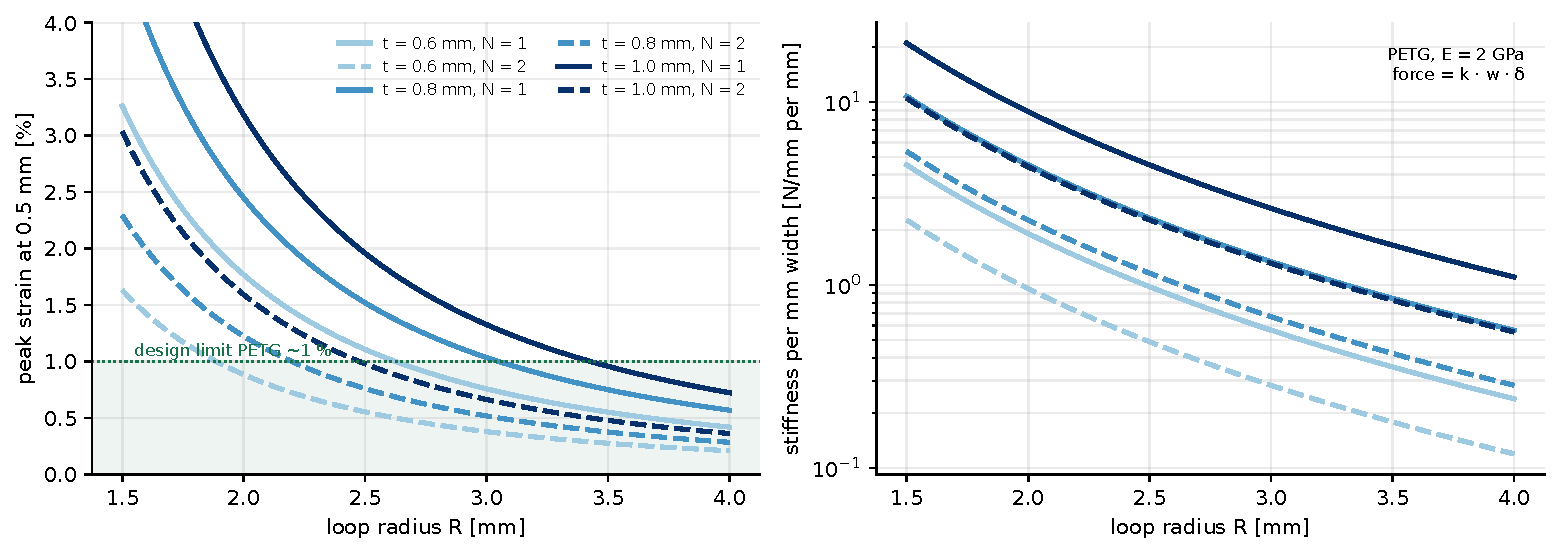
\includegraphics[width=\textwidth]{springs_loop}
\caption{C-loop design chart ($e=0$, \SI{270}{\degree}, PETG). Left: peak strain at
$\delta_\text{max}=\SI{0.5}{mm}$ picks $R$ for a given $t$ and number of loops $N$ (solid $N=1$,
dashed $N=2$); it does not depend on $w$ or $E$. Right: stiffness per millimetre of width; multiply
by $w$ and $\delta_0$ for the preload.}
\label{fig:loopchart}
\end{figure}

\begin{table}[H]\centering\small
\caption{C-loop options, PETG, $\delta_0=\SI{0.2}{mm}$, $\delta_\text{max}=\SI{0.5}{mm}$, $e=0$.
Red: above the strain limit. Arrow: the geometry in the drawings. The first row is the loop of an
earlier design: about three times stiffer than first estimated, and overstrained.}\label{tab:loop}
\begin{tabular}{c S[table-format=1.1] S[table-format=1.1] S[table-format=1.1] S[table-format=2.1] S[table-format=2.1] S[table-format=1.1] S[table-format=1.2] c}
\toprule
{$N$} & {$R$ [mm]} & {$t$ [mm]} & {$w$ [mm]} & {$J$ [mm$^2$]} & {$k$ [N/mm]} & {$F_0$ [N]} & {$\varepsilon_\text{max}$ [\%]} & \\
\midrule
\inputrows{generated/loop_table.tex}
\bottomrule
\end{tabular}
\end{table}

\paragraph{Printing the loop.}
\begin{itemize}
\item Print the loop module flat, loop plane in the build plane, so bending stays within layers.
\item Wall = whole extrusion lines; \SI{100}{\percent} infill is automatic at two lines. No
ironing or top skin across the loop.
\item Fillet the root (radius $\ge\SI{0.5}{mm}$): the root carries the largest moment.
\item Print it over-closed by $\delta_0$ (the jaw sits $\delta_0$ closer to the tooth than on the
model). Measure $F$ at $\delta_0$ and $\delta_\text{max}$; if needed change $w$, keep $t$ and $R$.
\item Polymers relax: after \SI{30}{min} at \SI{37}{\celsius} the force can be noticeably lower.
Size for the relaxed value, or accept re-printing.
\end{itemize}

% ---------------------------------------------------------------------------
\subsection{Straight clasp arm (alternative for concepts 1 and 2)}
A straight arm of length $L$ along the tooth, height $b$ and thickness $t$ (normal to the tooth),
clamped at the embrasure end:
\begin{equation}
k = \frac{E\,b\,t^3}{4L^3},\qquad \varepsilon_\text{max} = \frac{3\,t\,\delta_\text{max}}{2L^2}
\quad\Rightarrow\quad L \ge \sqrt{\frac{3\,t\,\delta_\text{max}}{2\,\varepsilon_\text{allow}}}.
\end{equation}
It lies flat against the lingual face and needs no tongue space, but a polymer arm that fits along
one molar gives little force (\cref{tab:arm}).
\begin{table}[H]\centering\small
\caption{Straight PETG clasp arm, $\delta_0=\SI{0.2}{mm}$, $\delta_\text{max}=\SI{0.5}{mm}$.}\label{tab:arm}
\begin{tabular}{S[table-format=2.0] S[table-format=1.0] S[table-format=1.1] S[table-format=1.1] S[table-format=1.1] S[table-format=1.2]}
\toprule
{$L$ [mm]} & {$b$ [mm]} & {$t$ [mm]} & {$k$ [N/mm]} & {$F_0$ [N]} & {$\varepsilon_\text{max}$ [\%]}\\
\midrule
\inputrows{generated/arm_table.tex}
\bottomrule
\end{tabular}
\end{table}

% ---------------------------------------------------------------------------
\subsection{Stainless arch wire (concept 4)}
Each leg of the arch is a cantilever from the rigid yoke to the molar pad, length
$L=\SI{17.6}{mm}$ (measured on the concept geometry), $E=\SI{185}{GPa}$:
\begin{equation}
k = \frac{3EI}{L^3},\quad I=\frac{\pi d^4}{64},\qquad F_0 = k\,\delta_0,\qquad
\sigma_\text{max} = \frac{3E\,(\delta_0+u)\,d/2}{L^2},
\end{equation}
and the pull-off force from \cref{eq:pulloff} with $z=\SI{3}{mm}$, $\mu=0.1$.

\begin{figure}[H]
\centering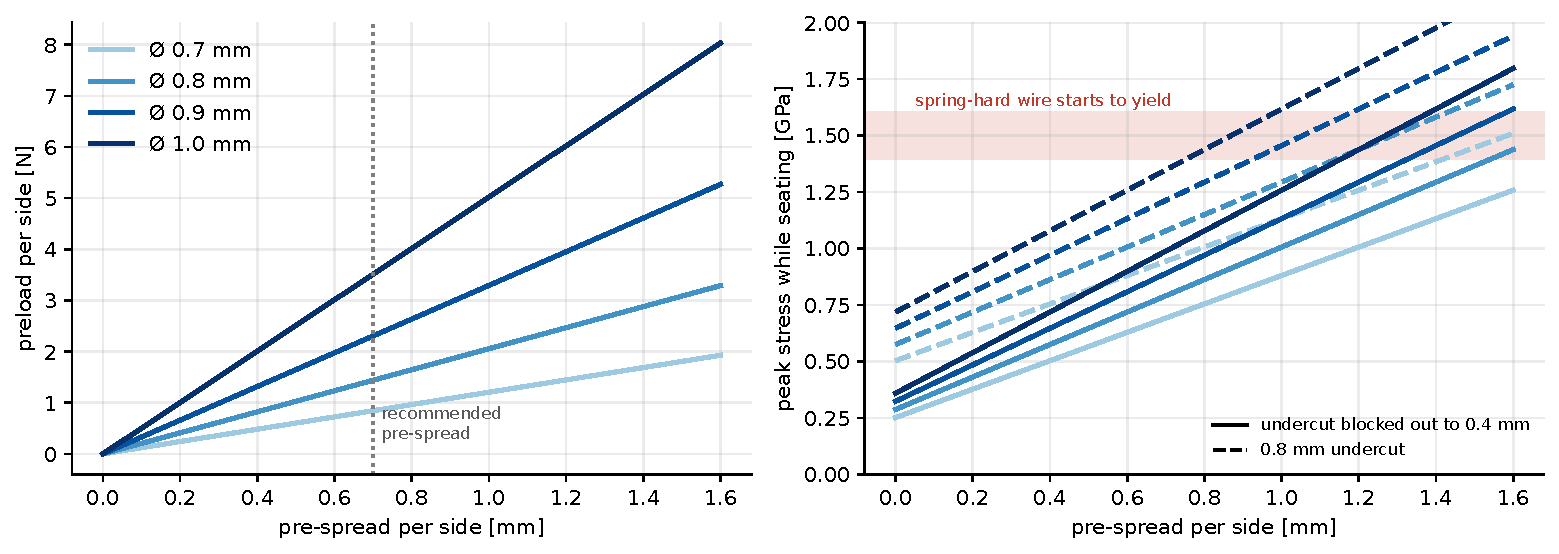
\includegraphics[width=\textwidth]{springs_wire}
\caption{Preload (left) and peak stress while seating (right) versus pre-spread. Red band: proof
stress of spring-hard wire (about \SIrange{1.4}{1.6}{GPa}).}
\label{fig:springs}
\end{figure}

\begin{table}[H]\centering\small
\caption{Arch wire, per side. Red: at or above the yield band.}\label{tab:wire}
\begin{tabular}{S[table-format=1.1] S[table-format=1.1] S[table-format=1.1] S[table-format=1.1] S[table-format=1.1] S[table-format=1.2] S[table-format=1.1]}
\toprule
{$d$ [mm]} & {$\delta_0$ [mm]} & {$u$ [mm]} & {$k$ [N/mm]} & {$F_0$ [N]} & {$\sigma_\text{max}$ [GPa]} & {$F_\text{pull-off}$ [N]}\\
\midrule
\inputrows{generated/wire_table.tex}
\bottomrule
\end{tabular}
\end{table}

\begin{keybox}
\textbf{The limit is stress, not force.} At fixed deflection the peak stress grows linearly with the
wire diameter, so a thicker wire yields \emph{sooner}. Use \textbf{\SI{0.9}{mm}, \SI{0.7}{mm}
pre-spread, undercut blocked out to \SI{0.4}{mm}}: \SI{\approx2.3}{N} preload, \SI{\approx0.9}{GPa}
peak. For the Adams clasps of concept~3, \SI{0.7}{mm} is the established size on permanent molars.
\end{keybox}

% ---------------------------------------------------------------------------
\subsection{TPU liner (concept 5)}
A liner of thickness $t_l$ squeezed by the interference $\delta$ over the contact area $A$:
\begin{equation}
F = E_c\,\varphi\,A\,\frac{\delta}{t_l},\qquad E_c \approx E\,(1+2\kappa S^2),\qquad S = \frac{A}{p\,t_l},
\end{equation}
with $\varphi$ the solid fraction of the liner, $p$ the perimeter of the loaded area, and the shape
factor $S$ stiffening a solid pad that cannot bulge sideways ($\kappa\approx0.6$--$0.9$). For the
contact band \SI{7}{mm}$\times$\SI{1.5}{mm} and $t_l=\SI{1.6}{mm}$ a solid pad has $E_c\approx1.8E$;
free-standing ribs have $E_c\approx E$. Tensile moduli \SI{12}{MPa} (85A) and \SI{26}{MPa} (95A).
\begin{table}[H]\centering\small
\caption{TPU liner force in N for a given interference.}\label{tab:tpu}
\begin{tabular}{l l S[table-format=2.0] S[table-format=2.0] S[table-format=2.0]}
\toprule
grade & liner & {\SI{0.1}{mm}} & {\SI{0.2}{mm}} & {\SI{0.3}{mm}}\\
\midrule
\inputrows{generated/tpu_table.tex}
\bottomrule
\end{tabular}
\end{table}
A ribbed 85A or 95A liner with \SIrange{0.1}{0.2}{mm} interference lands in the useful
\SIrange{3}{12}{N} range and tolerates print error; a solid liner is far too stiff and makes the
preload depend on hundredths of a millimetre. TPU moduli vary between brands: treat these numbers
as orders of magnitude.

% This file is part of JTS-MM (https://github.com/paulotto/jts-mm).
% SPDX-FileCopyrightText: 2026 Paul-Otto Müller
% SPDX-License-Identifier: CC-BY-4.0

\section{Fabrication workflow and tests}\label{sec:workflow}
\begin{enumerate}
\item \textbf{Get the dentition.} Intraoral scan of the lower arch, or an impression poured in stone
and scanned. Export STL; replace \texttt{../../scan/teeth\_02.stl} and re-run the scripts to get the
survey and concept geometry for this subject.
\item \textbf{Survey.} Pick the path of insertion that gives both first molars
\SIrange{0.3}{0.5}{mm} of lingual undercut (\texttt{s03\_survey.py}); block out deeper undercut;
add \SIrange{0.1}{0.2}{mm} relief elsewhere.
\item \textbf{Design.} Start from the concept STL in \texttt{stl/} or rebuild in CAD. Keep the rigid
reference, rests and marker mount as one stiff part; springs as separate, swappable parts where
possible.
\item \textbf{Print and assemble} (see each concept). Bench prototypes in PETG/PA12/TPU on a printed
model; parts for participants in certified splint resin.
\item \textbf{Fit on the model.} Seat, remove and re-seat; the part must click into place and sit on
its rests. Measure the spring force with a spring scale.
\item \textbf{Reline} the tooth-contacting hard surfaces with resin through the retention features.
\item \textbf{Fit in the mouth} under dental supervision: check the bite with articulating paper at
every embrasure crossing; check comfort, speech and tongue space.
\end{enumerate}

\paragraph{Acceptance tests.}
\begin{description}[style=nextline]
\item[Seating repeatability] Seat and remove the attachment ten times; measure the marker pose
relative to a tooth-fixed reference with the optical system each time. This is a measurement of
the system itself. A reasonable target is well below the
\SI{182}{\micro\metre} precision of the predecessor system.
\item[Pull-off force] Spring scale on the marker stem along the path of insertion. It must exceed
the loads during the protocol (lips, tongue, and sticky test foods if used).
\item[Stability under load] Log the marker pose while the participant chews; any drift relative to
the teeth shows up as a slow offset.
\item[Preload decay] Force after 0, 30 and \SI{60}{min} in \SI{37}{\celsius} water, for every
polymer spring.
\end{description}

% This file is part of JTS-MM (https://github.com/paulotto/jts-mm).
% SPDX-FileCopyrightText: 2026 Paul-Otto Müller
% SPDX-License-Identifier: CC-BY-4.0

\section{Materials and sources}\label{sec:procurement}
\begin{table}[H]\centering\small
\caption{Wire. The Amazon.de wire is the same alloy family as orthodontic wire but is sold as
craft wire, without a declaration of biocompatibility: use it for bench prototypes and bending
practice; use dental clasp wire for parts worn by participants.}
\begin{tabularx}{\textwidth}{l l X}
\toprule
use & wire & source\\
\midrule
concept 3 (Adams) & \SI{0.7}{mm} spring-hard stainless &
\href{https://www.amazon.de/Meter-Federstahldraht-0-7mm-Aisi-X10CrNi18-8/dp/B091PPTT8J}{Amazon.de, Federstahldraht 1.4310, 5\,m} (bench);
\href{https://www.dentalversender.de/Kieferorthopaedie/Draehte/remanium-Draht-Rolle-federhart-0-7-mm.html}{remanium\textsuperscript{\textregistered} federhart 0.7\,mm (DENTALVERSENDER)},
\href{https://www.dension-dental.de/produkt/remanium-stangendraht-packung-25-stueck-rund-federhart-o-070-mm/}{remanium\textsuperscript{\textregistered} straight lengths 0.70\,mm (Dension)},
\href{https://www.dension-dental.de/produkt/noninium-draht-rolle-draht-rund-federhart-o-07-mm/}{Noninium\textsuperscript{\textregistered} 0.7\,mm (Dension)}\\
concept 4 (arch) & \SI{0.9}{mm} spring-hard stainless &
\href{https://www.amazon.de/Meter-Federstahldraht-0-9mm-Aisi-X10CrNi18-8/dp/B091PQDL36}{Amazon.de, Federstahldraht 1.4310 0.9\,mm, 10\,m} or
\href{https://www.amazon.de/Meter-Federstahldraht-0-9mm-Aisi-X10CrNi18-8/dp/B091PQDYG3}{50\,m} (bench); dental clasp wire of the same diameter from the dental suppliers above\\
fallback & \SI{0.8}{mm} &
\href{https://www.amazon.de/Meter-Federstahldraht-0-8mm-Aisi-X10CrNi18-8/dp/B091PQBR9M}{Amazon.de, 0.8\,mm, 5\,m} (less preload, see \cref{tab:wire})\\
\bottomrule
\end{tabularx}
\end{table}

\paragraph{Checks for the Amazon wire.} The listing does not state a tensile class. Bend a test
piece to twice the planned deflection and check that it springs fully back. Never heat or solder
the wire: it loses its spring temper.

\paragraph{Other items.} Wire-bending pliers (a universal/Adams plier and a bird-beak plier);
light- or cold-curing reline resin; articulating paper; a small spring scale or force gauge
(\SIrange{0}{10}{N}); TPU 85A--95A filament; PETG or PA12 for frames; a certified splint resin for
parts worn by participants. Prices and stock were not checked.

\appendix
% This file is part of JTS-MM (https://github.com/paulotto/jts-mm).
% SPDX-FileCopyrightText: 2026 Paul-Otto Müller
% SPDX-License-Identifier: CC-BY-4.0

\section{Reproducing and editing the figures}\label{sec:reproduce}
Everything in this document is generated from \texttt{../../scan/teeth\_02.stl} by the scripts in
\texttt{scripts/}. Install the Python packages in \texttt{scripts/requirements.txt} and run
\texttt{scripts/run\_all.sh}; it rebuilds all figures, tables, STLs and this PDF (about
\SI{3}{min}; the 3D renders use VTK off-screen and need no display).

\begin{table}[H]\centering\small
\begin{tabularx}{\textwidth}{l X l}
\toprule
script & what it does & output\\
\midrule
\texttt{s00\_export\_teeth\_freecad.py} & optional, run with \texttt{freecadcmd}: exports \texttt{Teeth\_02} with its placement & \texttt{../../scan/}\\
\texttt{s01\_arch\_frame.py} & arch centreline, local frame, occlusal profile & \texttt{build/arch.npz}\\
\texttt{s02\_voxelize.py} & filled \SI{0.2}{mm} voxel model, distance field, arch coordinates & \texttt{build/field.npz}\\
\texttt{s03\_survey.py} & height of contour and undercut per tooth & \texttt{build/survey.json}, \cref{tab:survey}\\
\texttt{s04\_concepts.py} & the five concepts as voxel masks + wire paths, built from \texttt{params.py} & \texttt{stl/}, \texttt{build/concepts.pkl}\\
\texttt{s05\_render3d.py} & 3D renders, cameras in \texttt{CAMS} & \texttt{figures/png/render\_*}\\
\texttt{s06\_fig\_mechanics.py} & \cref{fig:mech,fig:undercut} & \texttt{mech\_*}\\
\texttt{s07\_fig\_sections.py} & first-molar sections of every concept & \texttt{section\_*}\\
\texttt{s08\_springs.py} & spring mathematics, \cref{fig:springs,fig:loopchart}, \cref{tab:wire,tab:loop,tab:tpu,tab:energy,tab:arm} & \texttt{springs\_*}, \texttt{generated/}\\
\texttt{s09\_drawings.py} & dimensioned drawings, reference dimensions, parameter tables & \texttt{drw\_*}, \texttt{generated/}\\
\texttt{s10\_export\_cad.py} & reference curves, stations, tooth sections and the FreeCAD macro & \texttt{cad/}\\
\texttt{params.py} & \textbf{every part dimension} (read by s04, s08, s09) & --\\
\bottomrule
\end{tabularx}
\end{table}

\paragraph{Editing figures.} Every 2D figure is written three times: \texttt{figures/svg/} (text is
kept as text, so labels can be edited in Inkscape or Illustrator), \texttt{figures/pdf/} (used by
this document) and \texttt{figures/png/} (preview). If you edit an SVG by hand, export it to PDF
under the same name (Inkscape: \emph{Save a Copy} $\rightarrow$ PDF) and LaTeX picks it up; but a
re-run of the scripts overwrites manual edits, so prefer changing the script where possible. The 3D
renders are PNG only: a vector export of \num{e5} triangles is neither small nor editable. To
change what they show, edit \texttt{params.py} (dimensions) or the masks in \texttt{s04\_concepts.py} or the camera in
\texttt{s05\_render3d.py}.

\paragraph{Coordinates.} $x$ mesio-distal, $y$ arch depth, $z$ tooth axis with the cusp tips at the
smallest $z$ (the frame of \texttt{Teeth\_02} in the FreeCAD files of the parts). The
scripts add $h$ (height below the lowest cusp tip), $s$ (arc length along the arch, 0 at the
midline) and $n$ (offset from the arch centreline, positive buccal). Every mask in
\texttt{s04\_concepts.py} is written in $s$, $n$, $h$ and the distance to the teeth.

\end{document}
